\documentclass[a4paper, 10pt]{article}
\usepackage[cm]{fullpage}
\usepackage{listingsutf8}
\usepackage{anyfontsize}
\usepackage[margin=1cm]{geometry}
\usepackage[usenames,dvipsnames]{xcolor}  %% Allow color names
\definecolor{codegreen}{rgb}{0,0.6,0}
\definecolor{codegray}{rgb}{0.5,0.5,0.5}
\definecolor{codepurple}{rgb}{0.58,0,0.82}
\definecolor{backcolour}{rgb}{1,1,1} %% White background
\definecolor{deepblue}{rgb}{0,0,0.5}
\definecolor{deepgreen}{rgb}{0,0.5,0}
\usepackage[colorlinks=true,linkcolor=blue]{hyperref}
\usepackage{fancyhdr}
\usepackage{graphicx}
\usepackage[final]{pdfpages}

\pagestyle{fancy}
\fancyhf{}
\lhead{University of the Basque Country - Team TrikiTriXa}
\rhead{Page \thepage}
\setlength{\headheight}{12pt}
\setlength{\headsep}{0.1in}

\fontsize{8pt}{10pt}

\begin{document}
\lstset{inputencoding=utf8/latin1}
\lstset{extendedchars=true}
\newcommand{\ProcessDigit}[1]{\bfseries \color{orange!75!black} #1}
\lstset{%
	backgroundcolor=\color{white},
	basicstyle=\footnotesize\ttfamily,
	commentstyle=\itshape\color{white!25!black},
	keywordstyle=\bfseries\color{deepblue},
	stringstyle=\color{deepgreen},
	identifierstyle=\color{orange!20!black},
	numbers=left,
	numbersep=5pt,
	numberstyle=\tiny\color{white!50!black},
	xleftmargin=0.5cm,
	tabsize=4,
	breaklines=true,
	literate=
	{0}{{{\ProcessDigit{0}}}}1
	{1}{{{\ProcessDigit{1}}}}1
	{2}{{{\ProcessDigit{2}}}}1
	{3}{{{\ProcessDigit{3}}}}1
	{4}{{{\ProcessDigit{4}}}}1
	{5}{{{\ProcessDigit{5}}}}1
	{6}{{{\ProcessDigit{6}}}}1
	{7}{{{\ProcessDigit{7}}}}1
	{8}{{{\ProcessDigit{8}}}}1
	{9}{{{\ProcessDigit{9}}}}1,
}
\setcounter{page}{20}
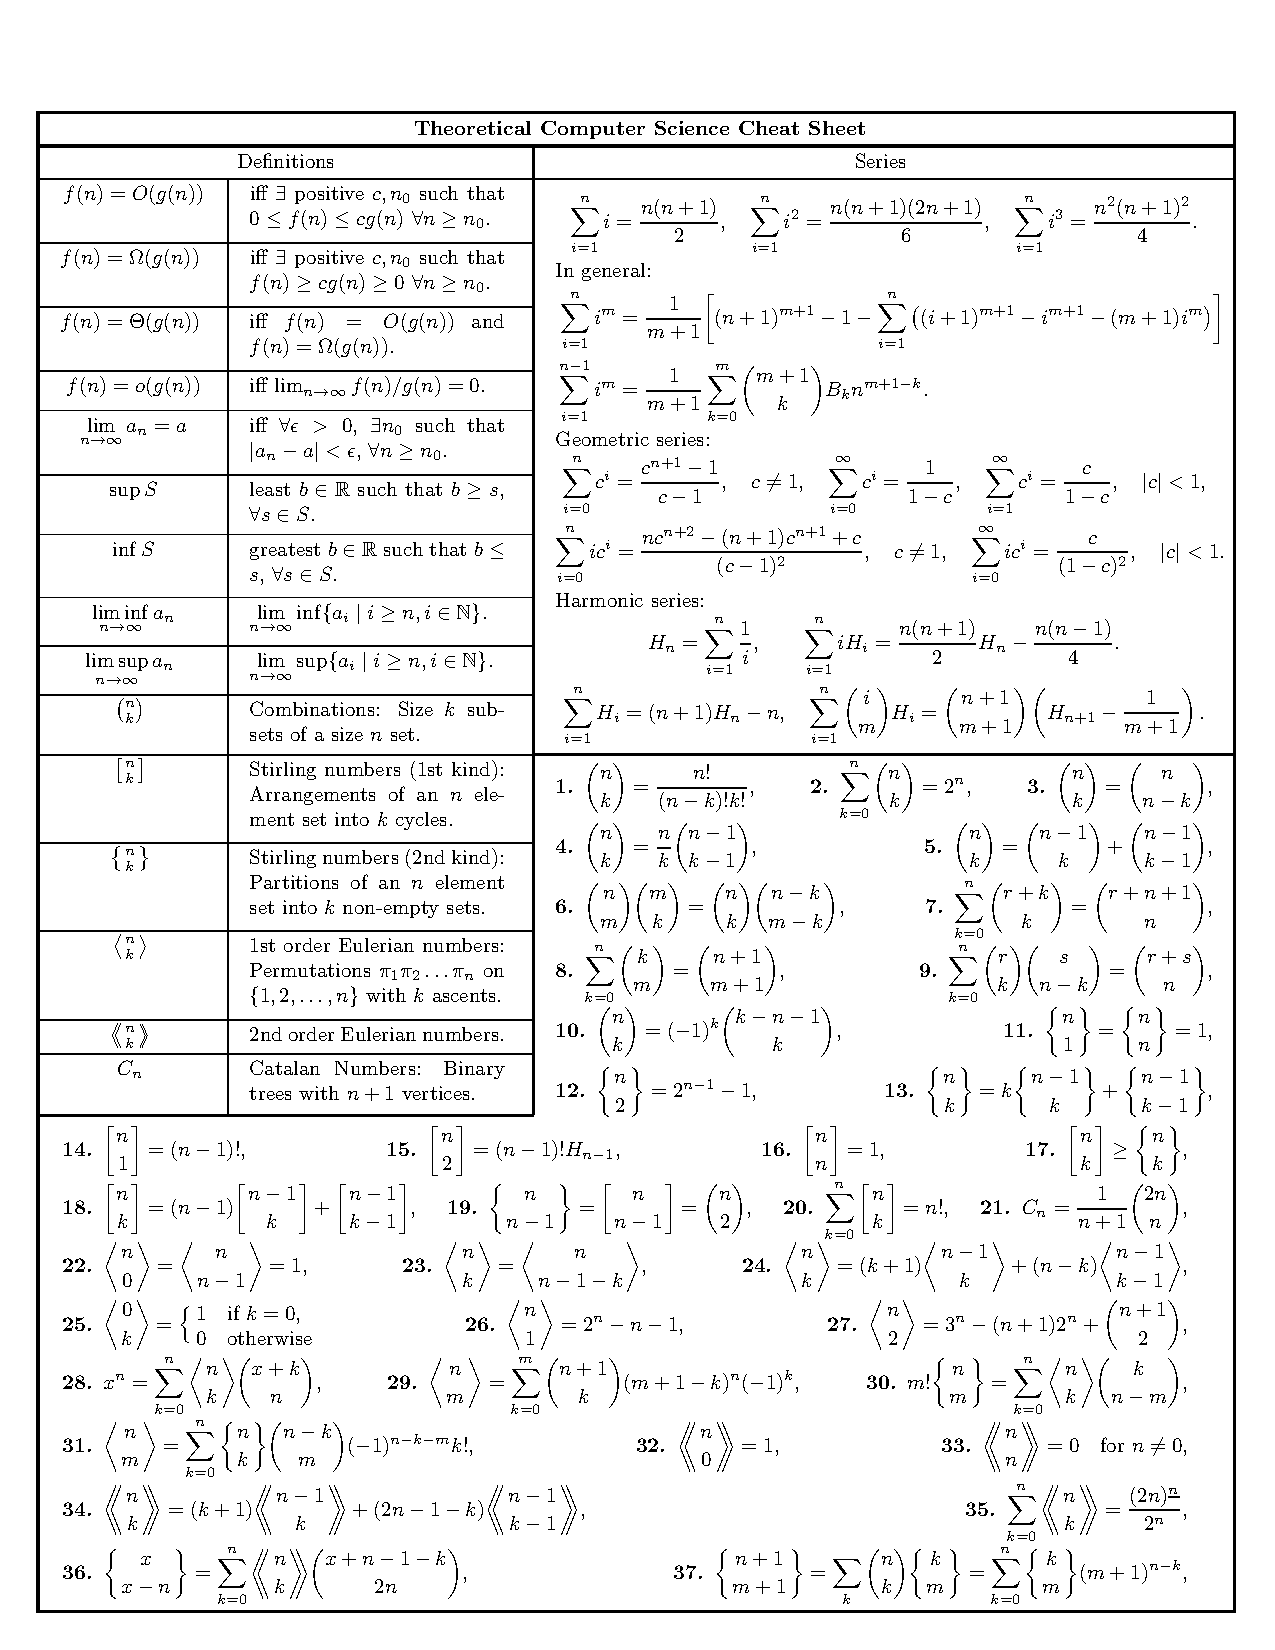
\includepdf[pages=-,pagecommand={},width=\textwidth]{notebook/cheatsheet.pdf}
\end{document}
